%%%%%%%%%%%%%%%%%%%%%%%%%%%%%%%%%%%%%%%%%%%%%%%%%%%%%%%%%%%%%%%%%%%%%%%%%%%%%%%%
% Operation
%%%%%%%%%%%%%%%%%%%%%%%%%%%%%%%%%%%%%%%%%%%%%%%%%%%%%%%%%%%%%%%%%%%%%%%%%%%%%%%%
\part{Operation} \label{Operation}

%%%%%%%%%%%%%%%%%%%%%%%%%%%%%%%%%%%%%%%%%%%%%%%%%%%%%%%%%%%%%%%%%%%%%%%%%%%%%%%%
% Modules
%%%%%%%%%%%%%%%%%%%%%%%%%%%%%%%%%%%%%%%%%%%%%%%%%%%%%%%%%%%%%%%%%%%%%%%%%%%%%%%%
\chapter{Modules} \label{Modules}

%%%%%%%%%%%%%%%%%%%%%%%%%%%%%%%%%%%%%%%%%%%%%%%%%%%%%%%%%%%%%%%%%%%%%%%%%%%%%%%%
% Modules - Introduction
%%%%%%%%%%%%%%%%%%%%%%%%%%%%%%%%%%%%%%%%%%%%%%%%%%%%%%%%%%%%%%%%%%%%%%%%%%%%%%%%
\section{Introduction}

There are a number of functions that the device performs.  Each set of
functionality will be called a \textit{module}.  There are some modules that are
always active and some that can only be active at one time.  Those that are
always active will be called \textit{components}.  Those that can only be active
at one time will be called \textit{modes}.

\begin{table}[H]
\ers{1}
\centering
\begin{tabu} { X[1,c,m] | X[1,c,m] }
  \thrule

  & \hyperref[Audio]{\mAu{s}} \\
  \thbi{Components} & \hyperref[Alarm]{\mAl{s}} \\
  & \hyperref[Power]{\mPo{s}} \\ \drule{2}

  & \hyperref[Clock]{\mCl{s}} \\
  & \hyperref[Set Alarm]{\mSA{s}}  \\
  & \hyperref[Timer]{\mTi{s}} \\
  \thbi{Modes} & \hyperref[Set Clock]{\mSC{s}} \\
  & \hyperref[Power Settings]{\mPS{s}} \\
  & \hyperref[Touch Settings]{\mTS{s}} \\
  & \hyperref[Set Night Light]{\mSN{s}} \\
  \bhrule
\end{tabu}
\caption {Modules}
\end{table}

%%%%%%%%%%%%%%%%%%%%%%%%%%%%%%%%%%%%%%%%%%%%%%%%%%%%%%%%%%%%%%%%%%%%%%%%%%%%%%%%
% Modules - State Diagrams
%%%%%%%%%%%%%%%%%%%%%%%%%%%%%%%%%%%%%%%%%%%%%%%%%%%%%%%%%%%%%%%%%%%%%%%%%%%%%%%%
\section{State Diagrams}

At the end of each module section will be a diagram showing the states it can be
in and the movement from one state to another and actions triggering the
movement.  The following table shows and describes the diagram elements.

\pagebreak

\ers{3}
\begin{longtabu}{ X[1,c,m] | X[5,l,m] }
  \thrule

  \thbi{Symbol} & \thbi{Meaning} \\ \mdrule

  \symMode{MODULE}
    & An element that is a \mode{sym}{MODULE}, i.e. a \mode{sym}{MODE}
      or \mode{sym}{COMPONENT}. \\ \mrule

  \symMenu{MENU}
    & An element that is a \menu{sym}{MENU} option available in certain modes.
      A menu state will contain a number options that will branch
      to different states. \\ \mrule

  \symState{STATE}
    & An element that is a \state{sym}{STATE} that a mode or
      component can be in. \\ \mrule

  \multirow{6}{*}{\symUnidirectional}
    & A \textit{unidirectional} or one-way path or flow from one element to
      the same or different element. \\ \dcrule{2}{2}
    & \parbox{\linewidth}{\centering \symUniModule \quad\quad \symUniMenu \quad\quad \symUniState} \\
    & \footnotesize{One or more actions may be associated
        with the path, i.e. will trigger the movement from one element
        to another. Either a symbol or text may be located next to or near
        the path line indicating the
        action that triggers the movement.} \\
    & \parbox{\linewidth}{\centering \symUniStateAction} \\ \dcrule{2}{2}
    & \footnotesize{A state can have a path that points to itself.
        There may be output or effects due to the action but
        the state does not change.} \\
    & \parbox{0.85\linewidth}{\centering \symUniSameState} \strut \\ \mrule

  \multirow{5}{*}{\symBidirectional}
    & A \textit{bidirectional} or two-way path or flow between two elements. \\ \dcrule{2}{2}
    & \footnotesize{One or more actions may be associated
        with the path, i.e will trigger the movement between the two
        elements. Either an action
        symbol or text will be located next to or near the path line
        indicating the action that triggers the movement.} \\
    & \parbox{\linewidth}{\centering \symBiStateOne} \\ \dcrule{2}{2}
    & \footnotesize{If there is more than one action associated
        with the path, the action \textit{nearest the arrow} is
        what determines the path or flow \textit{in the direction of the arrow}.} \\
    & \parbox{\linewidth}{\centering \symBiState} \\ \mrule

  \pagebreak
  \mrule

  \multirow{3}{*}{\symNode}
    & A \textit{node} that combines two or more unidirectional paths from two or
      more states into one unidirectional path to one state. \\ \dcrule{2}{2}
    & \footnotesize{Each path leading into the node will have an
        action associated with it.  The actions may be the same
        or different, but the resulting state will be the same.} \\
    & \parbox{\linewidth}{\centering \symNodeState} \strut \\

  \bhrule
\caption{State Diagram Symbols}
\end{longtabu}

%%%%%%%%%%%%%%%%%%%%%%%%%%%%%%%%%%%%%%%%%%%%%%%%%%%%%%%%%%%%%%%%%%%%%%%%%%%%%%%%
% Modules - Components
%%%%%%%%%%%%%%%%%%%%%%%%%%%%%%%%%%%%%%%%%%%%%%%%%%%%%%%%%%%%%%%%%%%%%%%%%%%%%%%%
\section{Components}

A component is a module that is enabled and running at all times unless
explicitly disabled.  Components all run and function concurrently and are
independent of any mode the device might be in.

\par\medskip

There are \num{3} components each described in individual sections.

\begin{table}[H]
\ers{4}
\centering
\begin{tabu}{ X[1,c,m] | X[3,l,m] }
  \thrule
  \thbi{Component} & \thbi{Description} \\ \mrule

  \hyperref[Audio]{\mAu{s}}
    & Provides the functionality related to track selection and
      playback. \\ \drule{2}
  \hyperref[Alarm]{\mAl{s}}
    & Contains the functionality related to alarm waking, snoozing and stopping
      and remains active in all power states. \\ \drule{2}
  \hyperref[Power]{\mPo{s}}
    & Governs device power states and when the device should nap, sleep or
      auto-stop the audio. \\
  \bhrule
\end{tabu}
\end{table}

%%%%%%%%%%%%%%%%%%%%%%%%%%%%%%%%%%%%%%%%%%%%%%%%%%%%%%%%%%%%%%%%%%%%%%%%%%%%%%%%
% Modules - Modes
%%%%%%%%%%%%%%%%%%%%%%%%%%%%%%%%%%%%%%%%%%%%%%%%%%%%%%%%%%%%%%%%%%%%%%%%%%%%%%%%
\section{Modes}

A mode is a device state containing specific functionality.  The device can be
in \textit{one and only one} mode at a time.  There are \num{7} modes each
described in individual sections.

\begin{table}[H]
\ers{4}
\centering
\begin{tabu}{ X[1,c,m] | X[3,l,m] }
  \thrule
  \thbi{Mode} & \thbi{Description} \\ \mrule

  \hyperref[Clock]{\mCl{s}}
    & Displays the time. Can display the date and current track.
    Provides direct selection of a track for playback. Is the only mode
    where the night light can be turned on and off. \\ \drule{2}
  \hyperref[Set Alarm]{\mSA{s}} & Set a time of day alarm that is used by
    the \hyperref[Alarm]{\mAl{s}} component. \\ \drule{2}
  \hyperref[Timer]{\mTi{s}} & Set and run a timer. \\ \drule{2}
  \hyperref[Set Clock]{\mSC{s}} & Set the time and date. \\ \drule{2}
  \hyperref[Power Settings]{\mPS{s}} & Settings related to power consumption
    that are used by the \hyperref[Power]{\mPo{s}} component. \\ \drule{2}
  \hyperref[Touch Settings]{\mTS{s}} & Settings related to the touch sensing
    capability of the device. \\ \drule{2}
  \hyperref[Set Night Light]{\mSN{s}} & Set any of the \num{3} configurable
    night light colors. \\

  \bhrule
\end{tabu}
\end{table}

Modes are selected using the \cRs{f} and the \cEs{f}.  They are partitioned
into \mPr{f}, \mSe{f} and \mTe{f}.

\begin{table}[H]
\ers{1}
\centering
\begin{tabu} { X[1,c,m] | X[1,c,m] }
  \thrule

  & \hyperref[Clock]{\mCl{s}} \\
  \hyperref[Primary Modes]{\mPr{s}} & \hyperref[Set Alarm]{\mSA{s}} \\
  & \hyperref[Timer]{\mTi{s}} \\ \drule{2}

  \multirow{2}{*}[-1mm]{\hyperref[Secondary Modes]{\mSe{s}}}
    & \hyperref[Set Clock]{\mSC{s}} \\
  & \hyperref[Power Settings]{\mPS{s}} \\ \drule{2}

  \multirow{2}{*}[-1mm]{\hyperref[Tertiary Modes]{\mTe{s}}}
    & \hyperref[Touch Settings]{\mTS{s}} \\
  & \hyperref[Set Night Light]{\mSN{s}} \\
  \bhrule
\end{tabu}
\caption {Modes}
\end{table}

The position of the \cRs{f} avails a subset of modes.  When the \cRs{f} is
turned, the \mPr{f} mode is automatically selected.  The \cEs{f} is then used
to select \mSe{f} and \mTe{f} modes.

%%%%%%%%%%%%%%%%%%%%%%%%%%%%%%%%%%%%%%%%%%%%%%%%%%%%%%%%%%%%%%%%%%%%%%%%%%%%%%%%
% Modules - Modes - Settings Modes
%%%%%%%%%%%%%%%%%%%%%%%%%%%%%%%%%%%%%%%%%%%%%%%%%%%%%%%%%%%%%%%%%%%%%%%%%%%%%%%%
\subsection{Settings Modes}

Settings that can change value will be \textit{blinking} on the \cDi{f}. If
there is more than one setting to configure on the \cDi{f} at a time as in the
case of setting a time or date, the one currently being set will be
\textit{blinking} on the \cDi{f}.

%%%%%%%%%%%%%%%%%%%%%%%%%%%%%%%%%%%%%%%%%%%%%%%%%%%%%%%%%%%%%%%%%%%%%%%%%%%%%%%%
% Modules - Modes - Modes Diagram
%%%%%%%%%%%%%%%%%%%%%%%%%%%%%%%%%%%%%%%%%%%%%%%%%%%%%%%%%%%%%%%%%%%%%%%%%%%%%%%%
\subsection{Modes Diagram}

The following diagram illustrates the modes of operation and the actions using
the \cRs{f} and \cEs{f} that lead to and from each mode.

\begin{figure}[H]
\centering
  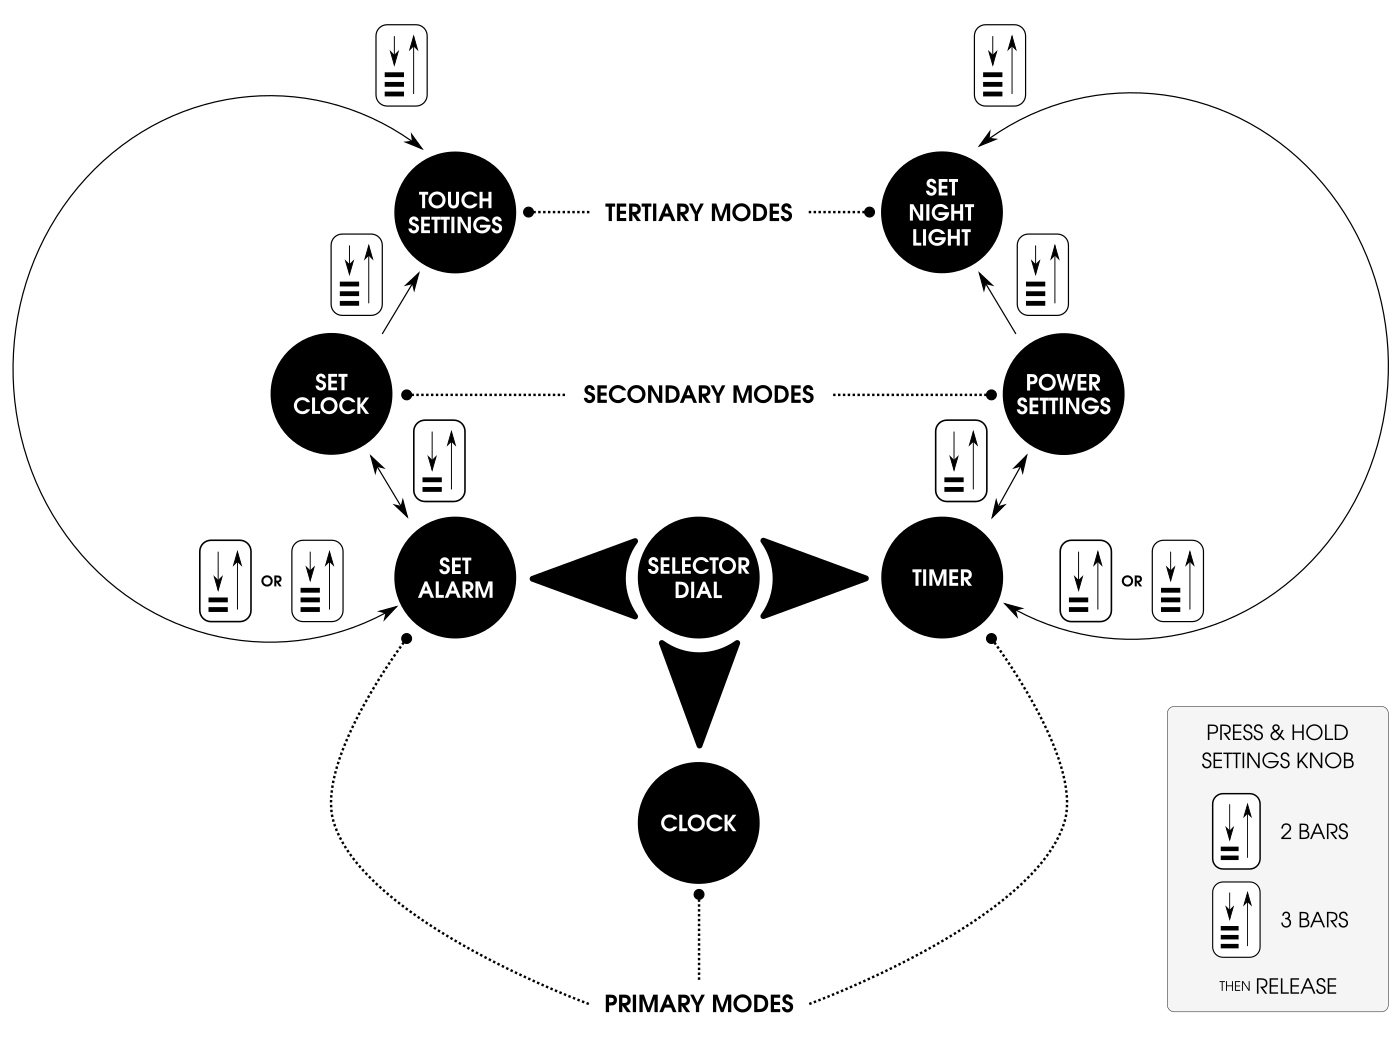
\includegraphics{images/modes_diagram.png}
\caption{Modes Diagram}
\end{figure}

%%%%%%%%%%%%%%%%%%%%%%%%%%%%%%%%%%%%%%%%%%%%%%%%%%%%%%%%%%%%%%%%%%%%%%%%%%%%%%%%
% Selector Dial
%%%%%%%%%%%%%%%%%%%%%%%%%%%%%%%%%%%%%%%%%%%%%%%%%%%%%%%%%%%%%%%%%%%%%%%%%%%%%%%%
\chapter{Selector Dial} \label{Operation - Selector Dial}

The \cRs{f} is used to select a subset of available modes.  The position
determines which modes are available.

\begin{table}[H]
\ers{2}
  \begin{tabu}{ X[1,c,m] | X[1,c,m] | X[1,c,m] | X[1,c,m] }  
    \thrule
    \multirow{2}{*}[-1mm]{\thbi{Position}}
      & \multicolumn{3}{c}{\thbi{Modes}} \\ \tabucline{2-4}

    & \mPr{n} & \mSe{n} & \mTe{n}
    \\ \hline

    \sLe & \hyperref[Set Alarm]{\mSA{s}}
      & \hyperref[Set Clock]{\mSC{s}}
      & \hyperref[Touch Settings]{\mTS{s}} \\ \drule{4}
    \sMi & \hyperref[Clock]{\mCl{s}} & --- & --- \\ \drule{4}
    \sRi & \hyperref[Timer]{\mTi{s}}
      & \hyperref[Power Settings]{\mPS{s}}
      & \hyperref[Set Night Light]{\mSN{s}} \\
  \bhrule
  \end{tabu}
\caption {Selector Dial - Positions \& Modes}
\end{table}

Turning the \cRs{f} will automatically set the mode to the \mPr{f} mode for the
given position.  The \hyperref[Operation - Settings Knob]{\cEs{f}} is then used
to select \mSe{f} and \mTe{f} modes.

\par\medskip

There are a number of symbols used to indicate turning actions.

\begin{table}[H]
\ers{5}
\centering
  \begin{tabu} { X[1,c,m] | X[3,l,m] }
    \thrule
    \thbi{Symbol} & \thbi{Meaning} \\ \mrule
    $\hskip -5.5mm$ \sMtoL & Turn from \dMi{f} to \dLe{f}. \\ \drule{2}
    $\hskip -5.5mm$ \sLtoM & Turn from \dLe{f} to \dMi{f}. \\ \drule{2}
    $\hskip 2.5mm$ \sMtoR & Turn from \dMi{f} to \dRi{f}. \\ \drule{2}
    $\hskip 2.5mm$ \sRtoM & Turn from \dRi{f} to \dMi{f}. \\ \drule{2}
    \sLtoR & Turn from \dLe{f} to \dRi{f}. \\ \drule{2}
    \sRtoL & Turn from \dRi{f} to \dLe{f}. \\
    \bhrule
  \end{tabu}
\end{table}

%%%%%%%%%%%%%%%%%%%%%%%%%%%%%%%%%%%%%%%%%%%%%%%%%%%%%%%%%%%%%%%%%%%%%%%%%%%%%%%%
% Settings Knob
%%%%%%%%%%%%%%%%%%%%%%%%%%%%%%%%%%%%%%%%%%%%%%%%%%%%%%%%%%%%%%%%%%%%%%%%%%%%%%%%
\chapter{Settings Knob} \label{Operation - Settings Knob}

The \cEs{f} is the primary control for interacting with the device.  It can be
\textit{turned} and \textit{pressed}.

%%%%%%%%%%%%%%%%%%%%%%%%%%%%%%%%%%%%%%%%%%%%%%%%%%%%%%%%%%%%%%%%%%%%%%%%%%%%%%%%
% Settings Knob - Turning
%%%%%%%%%%%%%%%%%%%%%%%%%%%%%%%%%%%%%%%%%%%%%%%%%%%%%%%%%%%%%%%%%%%%%%%%%%%%%%%%
\section{Turning}

There are \textit{no} start or stop positions when turning and it will turn
indefinitely in either direction.  While turning, you will notice bumps - termed
\textit{detents} - that provide a tactile feel for turning progression.

\par\medskip

In general, when setting values:

\begin{itemize}
  \item Turning \textit{clockwise} will \textit{increase} a value.
  \item Turning \textit{counter-clockwise} will \textit{decrease} a value.
  \item Values will \textit{change} at each \textit{detent}.
\end{itemize}

If you turn past a \textit{minimum} or \textit{maximum}, the value will usually
wrap or cycle.

\begin{itemize}
  \item If a value is at a \textit{maximum}, a \textit{clockwise} turn will
    circle to the \textit{minimum}.
  \item If a value is at a \textit{minimum}, a \textit{counter-clockwise} turn
    will circle to the \textit{maximum}.
\end{itemize}

\begin{figure}[H]
\centering
  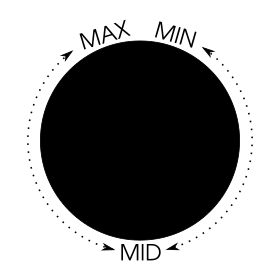
\includegraphics{images/settings_knob_wrap.png}
\caption{Settings Knob Turning}
\end{figure}

Note that the above figure is not a literal representation of where values will
lie in relation to the \cEs{f}.  You may have to turn the knob for only a couple
of detents to reach a midpoint value or cycle through all of the allowable
values.  Or you may have to turn for many revolutions.  It is meant to show that
values are arranged circularly as opposed to linearly.

\par\medskip

Consider, for example, setting a minute or second value, where the allowable
range is \mono{0-59}.  If the current value is \num{59}, a clockwise turn will
cycle to \num{0}.  Likewise if the current value is \num{0}, a counter-clockwise
turn will cycle to \num{59}.

\begin{figure}[H]
\centering
  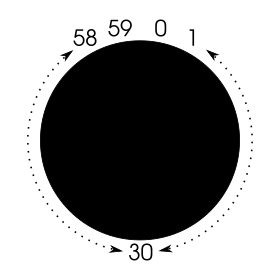
\includegraphics{images/settings_knob_wrap_example.png}
\end{figure}

\info{It can often be quicker to turn in the opposite direction to get to a
value.}

\par\medskip

There are a number of symbols that will be used indicating direction, number of
times, not to turn or a failure to turn within a specified amount of time.

\begin{table}[H]
\ers{2}
\centering
  \begin{tabu}{ X[1,c,m] | X[4,l,m] }
  \thrule

  \thbi{Symbol} & \thbi{Meaning} \\ \mrule

  \sTu & Turn in \textit{any} direction. \\ \drule{2}
  \sCl & Turn \textit{clockwise}. \\ \drule{2}
  \sCC & Turn \textit{counter-clockwise}. \\ \drule{2}
  \multirow{2}{*}[-1mm]{$\hskip 3.3mm$ \sTuN{$N$}}
    & Turn for at least $N$ detents in any direction. \\
  & \quad \sTuN{3} $\longrightarrow$ Turn until at least \num{3} detents
    are felt. \\ \drule{2}
  \multirow{2}{*}[-1mm]{$\hskip 3.3mm$ \sTuN{$N$s}} & Turn \textit{within}
    $N$ seconds. \\
  & \quad \sTuN{3s} $\longrightarrow$ Turn within \num{3} seconds. \\ \drule{2}
  \sNTu & Do \textit{not} turn. \\ \drule{2}
  \multirow{2}{*}[-1mm]{$\hskip 4.4mm$ \sNTuN{$N$}} & Failure to turn
    \textit{within} $N$ seconds. \\
  & \quad \sNTuN{15} $\longrightarrow$ Failure to turn within \num{15}
    seconds. \\
  \bhrule
  \end{tabu}
\caption{Settings Knob - Turn Symbols}
\end{table}

When the \cEs{f} is turned, you will feel bumps.  These are called
\textit{detents}.  When it is specified to turn $N$ times, it means detents
and \textit{not} full rotations.  So \enspace \sTuN{3} means to turn for at
least \num{3} bumps/detents.

%%%%%%%%%%%%%%%%%%%%%%%%%%%%%%%%%%%%%%%%%%%%%%%%%%%%%%%%%%%%%%%%%%%%%%%%%%%%%%%%
% Settings Knob - Pressing
%%%%%%%%%%%%%%%%%%%%%%%%%%%%%%%%%%%%%%%%%%%%%%%%%%%%%%%%%%%%%%%%%%%%%%%%%%%%%%%%
\section{Pressing}

There are \num{3} main pressing actions.

\begin{table}[H]
\ers{5}
\begin{tabu}{ X[2,c,m] | X[1,c,m] | X[4,l,m] }
  \thrule
  \thbi{Action} & \thbi{Abbr.} & \thbi{Description} \\ \mrule
  \hyperref[Press and Release]{\aPR{s}}
    & \fontTGA{s}{P\&R} & A relatively quick press \& release
    similar to a computer mouse click. \\ \drule{3}
  \hyperref[Double-Click]{\aDC{s}}
    & \fontTGA{s}{DC} & Press \& release \textit{twice} in quick
    succession, similar to a computer mouse double-click. \\ \drule{3}
  \hyperref[Press and Hold]{\aPH{s}}
    & \fontTGA{s}{P\&H} & Press and hold for some amount of time,
    then release. \\
  \bhrule
\end{tabu}
\caption {Settings Knob Pressing Actions}
\end{table}

%%%%%%%%%%%%%%%%%%%%%%%%%%%%%%%%%%%%%%%%%%%%%%%%%%%%%%%%%%%%%%%%%%%%%%%%%%%%%%%%
% Settings Knob - Pressing - Press & Release
%%%%%%%%%%%%%%%%%%%%%%%%%%%%%%%%%%%%%%%%%%%%%%%%%%%%%%%%%%%%%%%%%%%%%%%%%%%%%%%%
\subsection{Press \& Release} \label{Press and Release}

What action this performs will be dependent on context.

\par\medskip

In settings modes, it generally caches a setting and moves to the next setting
or if at the last setting, sets and saves all cached settings and finishes.

\par\medskip

In other cases, it may turn the alarm off, show the date or pause the timer.

\par\medskip

There are a number of symbols that will be used indicating number of times, not
to press or a failure to press within a specified amount of time.

\begin{table}[H]
\ers{2}
\centering
\begin{tabu}{ X[1,c,m] | X[5,l,m] }
  \thrule
  \thbi{Symbol} & \thbi{Meaning} \\ \mrule
  \sPR & Press \& release \textit{once}. \\ \drule{2}
  \multirow{2}{*}[-1mm]{$\hskip 3.3mm$ \sPRN{$N$}} & Press \& release $N$ times. \\
    & \quad \sPRN{4} $\longrightarrow$ Press \& release \num{4} times. \\ \drule{2}
  \multirow{2}{*}[-1mm]{$\hskip 3.3mm$ \sPRN{$N$s}}
    & Press \& release \textit{within} $N$ seconds. \\
    & \quad \sPRN{4s} $\longrightarrow$ Press \& release within \num{4} seconds. \\ \drule{2}
  \sNPR & Do \textit{not} press \& release. \\ \drule{2}
  \multirow{2}{*}[-1mm]{$\hskip 4.3mm$ \sNPRN{$N$}} & Failure to press \& release
    \textit{within} $N$ seconds. \\
    & \quad \sNPRN{3} $\longrightarrow$ Failure to press \& release within \num{3} seconds. \\
  \bhrule
\end{tabu}
\caption{Settings Knob - Press \& Release Symbols}
\end{table}

%%%%%%%%%%%%%%%%%%%%%%%%%%%%%%%%%%%%%%%%%%%%%%%%%%%%%%%%%%%%%%%%%%%%%%%%%%%%%%%%
% Settings Knob - Pressing - Double-Click
%%%%%%%%%%%%%%%%%%%%%%%%%%%%%%%%%%%%%%%%%%%%%%%%%%%%%%%%%%%%%%%%%%%%%%%%%%%%%%%%
\subsection{Double-Click} \label{Double-Click}

This is currently only used in \hyperref[Set Night Light]{\mSN{f}} and has one
associated symbol.

\begin{table}[H]
\ers{2}
\centering
\begin{tabu}{ X[1,c,m] | X[5,l,m] }
  \thrule
  \thbi{Symbol} & \thbi{Meaning} \\ \mrule
  \sDC & Press \& release \textit{twice} in quick succession. \\
  \bhrule
\end{tabu}
\caption {Settings Knob - Double-Click Symbol}
\end{table}

It is distinguished from \enspace \sPRN{$N$} in that the second press \& release
\textit{must} be done very quickly - within \mono{300\thinspace ms} which is
a little less than $\frac{1}{3}$ of a second.

%%%%%%%%%%%%%%%%%%%%%%%%%%%%%%%%%%%%%%%%%%%%%%%%%%%%%%%%%%%%%%%%%%%%%%%%%%%%%%%%
% Settings Knob - Pressing - Press & Hold
%%%%%%%%%%%%%%%%%%%%%%%%%%%%%%%%%%%%%%%%%%%%%%%%%%%%%%%%%%%%%%%%%%%%%%%%%%%%%%%%
\subsection{Press \& Hold} \label{Press and Hold}

This pressing action will, in general, do one of the following:

\begin{itemize}
  \item \aReset{f} a settings mode, i.e. allow starting over from the
    beginning or some origin state.
  \item Go to \mSe{f} or \mTe{f} modes -
    see \hyperref[Operation - Selector Dial]{\cRs{f}}.
  \item If currently in a \mSe{f} or \mTe{f} mode, go back to the \mPr{f} mode.
\end{itemize}

In every mode except \mCl{f} mode, bars / dashes will be shown and blink on the
\cDi{s} providing a visual indication to release.

\begin{table}[H]
\ers{3}
\begin{tabu}{ X[1,c,m] | X[1,c,m] | X[1,c,m] }
  \thrule
  \thbi{Display} & \thbi{Hold Time} & \thbi{Effect} \\ \mrule
  \sDl{<<<<} & \num{1.5} seconds & \aReset{f} \\ \drule{3}
  \sDl{====} & \num{4.0} seconds
    & \multirow{2}{*}[-1mm]{\action{f}{CHANGE MODE}} \\ \drule{2}
  \sDl{>>>>} & \num{6.5} seconds \\
  \bhrule
\end{tabu}
\caption{Settings Knob - Press \& Hold}
\end{table}

The following table shows the mode changes when the \cEs{f} is pressed and held
for two or three bars.

\begin{table}[H]
\ers{3}
\begin{tabu}{ X[1,c,m] | X[1,c,m] | X[1,c,m] }
  \thrule
  \thbi{Mode} & \thbi{Display} & \thbi{Next} \\ \mrule

  \multirow{2}{*}[-1mm]{\mPr{n}} & \sDl{====} & \mSe{n} \\ \dcrule{2}{3}
  & \sDl{>>>>} & \mTe{n} \\ \mrule

  \multirow{2}{*}[-1mm]{\mSe{n}} & \sDl{====} & \mPr{n} \\ \dcrule{2}{3}
  & \sDl{>>>>} & \mTe{n} \\ \mrule

  \multirow{2}{*}[-1mm]{\mTe{n}} & \sDl{====}
    & \multirow{2}{*}[-1mm]{\mPr{n}} \\ \dcrule{2}{2}
  & \sDl{>>>>} & \\
  \bhrule
\end{tabu}
\caption{Settings Knob - Press \& Hold Modes}
\end{table}

For example, to go to \hyperref[Touch Settings]{\mTS{f}} which is a \mTe{f} mode
and assuming the \cRs{f} is \textit{not} already pointing to the \dLe{f}:

\begin{enumerate}
  \item \aTu{f} the \cRs{f} to the \dLe{f}.
  \item \aPH{f} the \cEs{f} until you see \symD{>>>>} blink on the \cDi{f}.
  \item \aRe{f} the \cEs{f}.
\end{enumerate}

To go back to \hyperref[Set Alarm]{\mSA{f}} which is a \mPr{f} mode:

\begin{enumerate}
  \item \aPH{f} the \cEs{f} until you see \symD{====} or \symD{>>>>}
    blink on the \cDi{f}.
  \item \aRe{f} the \cEs{f}.
\end{enumerate}

There are a number of symbols that will be used indicating press type and
duration.

\begin{table}[H]
\ers{2}
\centering
\begin{tabu}{ X[1,c,m] | X[5,l,m] }
  \thrule
  \thbi{Symbol} & \thbi{Meaning} \\ \mrule
  \multirow{2}{*}[-1mm]{$\hskip 3.3mm$ \sPHN{$N$}}
    & Press \& hold for $N$ seconds then release. \\
    & \quad \sPHN{6} $\longrightarrow$ Press \& hold for \num{6} seconds then release. \\ \drule{2}
  \sReset & Press \& hold until \symD{<<<<} is displayed, then release. \\ \drule{2}
  \sSec & Press \& hold until \symD{====} is displayed, then release. \\ \drule{2}
  \sTer & Press \& hold until \symD{>>>>} is displayed, then release. \\
  \bhrule
\end{tabu}
\caption {Settings Knob - Press \& Hold Symbols}
\end{table}

%%%%%%%%%%%%%%%%%%%%%%%%%%%%%%%%%%%%%%%%%%%%%%%%%%%%%%%%%%%%%%%%%%%%%%%%%%%%%%%%
% Touch Sensor
%%%%%%%%%%%%%%%%%%%%%%%%%%%%%%%%%%%%%%%%%%%%%%%%%%%%%%%%%%%%%%%%%%%%%%%%%%%%%%%%
\chapter{Touch Sensor} \label{Operation - Touch Sensor}

The \cTS{f} utilizes
\href{https://en.wikipedia.org/wiki/Capacitive\_sensing}{Capacitive Touch Sensing}
which measures changes in capacitance of an \textit{electrode} to detect touch
events.  There are a number of functions that the \cTS{f} provides.

\begin{table}[H]
\centering
\ers{0.1}
\begin{tabu} { X[3,l,m] | X[2,c,m] }
  \thrule
  \thbi{Function} & \thbi{Module} \\ \mrule
  Snooze alarm. & \hyperref[Alarm]{\mAl{f}} \\ \drule{2}
  Show current track number. & \hyperref[Clock]{\mCl{f}} \\ \drule{2}
  Stop timer alerting. & \hyperref[Timer]{\mTi{f}} \\ \drule{2}
  Wake the device from nap or sleep. & \hyperref[Power]{\mPo{f}} \\ \drule{2}
  Toggle timer lighting on/off. & \hyperref[Timer]{\mTi{f}} \\ \drule{2}
  Forcibly put the device to sleep. & \hyperref[Power]{\mPo{f}} \\
  \bhrule
\end{tabu}
\end{table}

All of the above, except for the last two, can also be done using the \cEs{f},
so if you want or need to disable the \cTS{f} you will not lose much
functionality.

\par\medskip

When using the touch functionality, it is not enough to simply tap the top
with your index finger.  You \textit{must} place your \textit{hand} or the
majority of your fingers, palm down on the \cTo{f} of the enclosure.
The figure below shows the general amount of coverage.

\begin{figure}[H]
\centering
  
\includegraphics{images/touch_hand_coverage.png}
\caption{Touch Sensor - Hand Coverage} \label{fig:Hand Coverage}
\end{figure}

See \hyperref[Touch Settings]{\mTS{f}} for more information on configuring and
calibrating the \cTS{f}.

\par\medskip

There are a number of symbols that will be used indicating touch, touch
duration, not to touch and failure to touch within some amount of
time.\footnote{ Though an outstretched index finger is used in the symbol, the
palm of the hand or a majority of the fingers must be used.}

\begin{table}[H]
\ers{2}
\begin{tabu}{ X[1,c,m] | X[4,l,m] }
  \thrule
  \thbi{Symbol} & \thbi{Meaning} \\ \mrule
  \sTo & Touch the top of the enclosure with palm of hand. \\ \drule{2}
  \multirow{2}{*}[-1mm]{$\hskip 3.0mm$ \sToN{$N$}} & Touch for $N$ seconds. \\
    & \quad \sToN{5} $\longrightarrow$ Touch for \num{5} seconds. \\ \drule{2}
  \sNTo & Do \textit{not} touch. \\ \drule{2}
  \multirow{2}{*}[-1mm]{$\hskip 3.0mm$ \sNToN{$N$}}
    & Failure to touch \textit{within} $N$ seconds. \\
    & \quad \sNToN{3} $\longrightarrow$ Failure to touch within \num{3} seconds. \\ \drule{2}
  \bhrule
\end{tabu}
\caption {Touch Sensor Symbols}
\end{table}

%%%%%%%%%%%%%%%%%%%%%%%%%%%%%%%%%%%%%%%%%%%%%%%%%%%%%%%%%%%%%%%%%%%%%%%%%%%%%%%%
% Symbols
%%%%%%%%%%%%%%%%%%%%%%%%%%%%%%%%%%%%%%%%%%%%%%%%%%%%%%%%%%%%%%%%%%%%%%%%%%%%%%%%
\chapter{Symbols}

In addition to expository language, symbols will often be used to describe
actions and effects so that one can quickly surmise an action and outcome.

\par\medskip

For example, the following steps used in \mSC{f}:

\begin{enumerate}
  \item From the \sSCHo{f} state, \aTu{f} the \cEs{f} to select an hour.
  \item \aPR{f} the \cEs{f} to cache the selected hour and proceed to the
    \sSCMi{f} state.
\end{enumerate}

can be summed up using the following sequence of symbols:

\as{{c c c c}}{%
\sSCHo{sym} & \sTu & \sPR & \sSCMi{sym} \\}

Often, an \textit{effect} will be grouped with the \textit{action}:

\as{{c c c c}}{%
\multirow{2}{*}{\sSCHo{sym}}
  & \sTu & \sPR & \multirow{2}{*}{\sSCMi{sym}} \\
& \eUp{sym}{} & \eCa{sym}{} & \\}

And sometimes multiple actions will be grouped into one column indicating
that \textit{any} one of the actions can bring about the change.  For example,
the following is used in \mCl{f} to indicate any of three actions, or rather
inactions, that will cause the \sClSh{f} state to go back to the \sClTi{f}
state.

\as{{ c l l }}{%
& \sNTuN{3} & \\ \dcrule{2}{2}
\sClSh{sym} & \sNToN{3} & \sClTi{sym} \\ \dcrule{2}{2}
& \sNPRN{15} & \\}

\pagebreak

The table below sums up all of the symbols described in the previous sections.

\ers{3}
\begin{longtabu}{ X[1,c,m] | X[4,l,m] }
  \thrule
  \multicolumn{2}{c}{\textbf{\cRs{n}}} \\ \mrule
  \thbi{Symbol} & \thbi{Meaning} \\ \mrule
  $\hskip -5.5mm$ \sMtoL & Turn from \dMi{f} to \dLe{f}. \\ \drule{2}
  $\hskip -5.5mm$ \sLtoM & Turn from \dLe{f} to \dMi{f}. \\ \drule{2}
  $\hskip 2.5mm$ \sMtoR & Turn from \dMi{f} to \dRi{f}. \\ \drule{2}
  $\hskip 2.5mm$ \sRtoM & Turn from \dRi{f} to \dMi{f}. \\ \drule{2}

  \sLtoR & Turn from \dLe{f} to \dRi{f}. \\ \drule{2}
  \sRtoL & Turn from \dRi{f} to \dLe{f}. \\

  \thrule
  \multicolumn{2}{c}{\textbf{\cEs{n}}} \\ \mrule
  \thbi{Symbol} & \thbi{Meaning} \\ \mrule

  \sTu & Turn in \textit{any} direction. \\ \drule{2}
  \sCl & Turn \textit{clockwise}. \\ \drule{2}
  \sCC & Turn \textit{counter-clockwise}. \\ \drule{2}
  \multirow{2}{*}[-1mm]{$\hskip 3.3mm$ \sTuN{$N$}}
    & Turn for at least $N$ detents in any direction. \\
    & \quad \sTuN{3} $\longrightarrow$ Turn until at least \num{3} detents are felt. \\ \drule{2}

  \pagebreak
  \drule{2}

  \sNTu & Do \textit{not} turn. \\ \drule{2}
  \multirow{2}{*}[-1mm]{$\hskip 4.4mm$ \sNTuN{$N$}}
    & Failure to turn \textit{within} $N$ seconds. \\
    & \quad \sNTuN{15} $\longrightarrow$ Failure to turn within \num{15} seconds. \\ \drule{2}

  \sPR & Press \& release \textit{once}. \\ \drule{2}
  \multirow{2}{*}[-1mm]{$\hskip 3.3mm$ \sPRN{$N$}} & Press \& release $N$ times. \\
    & \quad \sPRN{4} $\longrightarrow$ Press \& release \num{4} times. \\ \drule{2}
  \sNPR & Do \textit{not} press \& release. \\ \drule{2}

  \multirow{2}{*}[-1mm]{$\hskip 4.3mm$ \sNPRN{$N$}}
    & Failure to press \& release \textit{within} $N$ seconds. \\
    & \quad \sNPRN{3} $\longrightarrow$ Failure to
      press \& release within \num{3} seconds. \\ \drule{2}

  \sDC & Press \& release \textit{twice} in quick succession. \\ \drule{2}

  \multirow{2}{*}[-1mm]{$\hskip 3.3mm$ \sPHN{$N$}}
    & Press \& hold for $N$ seconds then release. \\
    & \quad \sPHN{6} $\longrightarrow$ Press \& hold for \num{6} seconds then release. \\ \drule{2}
  \sReset & Press \& hold until \symD{<<<<} is displayed, then release. \\ \drule{2}
  \sSec & Press \& hold until \symD{====} is displayed, then release. \\ \drule{2}
  \sTer & Press \& hold until \symD{>>>>} is displayed, then release. \\

  \mrule
  \pagebreak

  \thrule
  \multicolumn{2}{c}{\textbf{\cTS{n}}} \\ \mrule
  \thbi{Symbol} & \thbi{Description} \\ \mrule

  \sTo & Touch the top of the enclosure with palm of hand. \\ \drule{2}

  \multirow{2}{*}[-1mm]{$\hskip 3.0mm$ \sToN{$N$}} & Touch for $N$ seconds. \\
    & \quad \sToN{5} $\longrightarrow$ Touch for \num{5} seconds. \\ \drule{2}
  \sNTo & Do \textit{not} touch. \\ \drule{2}
  \multirow{2}{*}[-1mm]{$\hskip 3.0mm$ \sNToN{$N$}}
    & Failure to touch \textit{within} $N$ seconds. \\
    & \quad \sNToN{3} $\longrightarrow$ Failure to touch within \num{3} seconds. \\

  \bhrule
\caption{Symbols - Reference}
\end{longtabu}
